\documentclass[12pt,twoside]{article}
\usepackage[dvipsnames]{xcolor}
\usepackage{tikz,graphicx,amsmath,amsfonts,amscd,amssymb,bm,cite,epsfig,epsf,url}
\usepackage[hang,flushmargin]{footmisc}
\usepackage[colorlinks=true,urlcolor=blue,citecolor=blue]{hyperref}
\usepackage{amsthm,multirow,wasysym,appendix}
\usepackage{array,subcaption} 
% \usepackage[small,bf]{caption}
\usepackage{bbm}
\usepackage{pgfplots}
\usetikzlibrary{spy}
\usepgfplotslibrary{external}
\usepgfplotslibrary{fillbetween}
\usetikzlibrary{arrows,automata}
\usepackage{thmtools}
\usepackage{blkarray} 
\usepackage{textcomp}

\usepackage[left=0.8in,right=1.0in,top=1.0in,bottom=1.0in]{geometry}
\newcommand{\red}[1]{{\leavevmode\color{red}{#1}}}
\newcommand{\blue}[1]{{\leavevmode\color{blue}{#1}}}
\usepackage{graphicx}
\input{macros}

\begin{document}

\begin{center}
{\large{\textbf{Homework 3}} } \vspace{0.2cm}\\
Due October 2 at 11 pm
\\
\end{center}
\input{hwstatement.tex}\\

\begin{enumerate}

\item (Fish)
A biologist is studying a rare species of fish. She captures four individuals and measures their weights, which are 5, 8, 5 and 6 kg.
\begin{enumerate}
\item
What is the empirical conditional probability that a fish weighs more than 7 kg given that they weigh more than 6 kg? 
\blue{
\begin{itemize}
    \item we could solve for P(fish weighs more than 7k given it weighs more than 6kg) as $\frac{\text{ weigh More than 7kg and weigh more than 6kg}}{\text{ weigh more than 6 kg}}=\frac{1}{1}=1$ so there is a 100$\%$ according to the empirical estimate
\end{itemize}
}

\item Plot an estimate of the pdf of the fish weight using kernel density estimation with a rectangular kernel of width 2. plot the bins as discrete .
\blue{
\begin{itemize}
  \includegraphics[width=15cm]{homework 3/temp 2 .png}
\end{itemize}
}
\item What is the conditional probability that a fish weighs more than 7 kg given that they weigh more than 6 kg according to your estimated pdf?
\end{enumerate}
\blue{
\begin{itemize}
    \item again we have $\frac{\text{ weigh More than 7kg and weigh more than 6kg}}{\text{ weigh more than 6 kg}}=\frac{\text{ weigh More than 7kg}}{\text{ weigh more than 6 kg}}$
    \item if we look at the area of fish that weigh more than 7, we can see it is 
    \frac{2}{8}
    \item if we look at the area of the pdf greater than 6 we can see that the area is \frac{3}{87}
    \item thus the ratio is $\frac{2}{3}$
    \item note that here i used area calculations instead of integrating as our pdf in this case is not continuous 
\end{itemize}}
\newpage

\item (Nuclear power plant)
The random variable $\rt$ with the following pdf
\begin{figure}[h]
\begin{center}
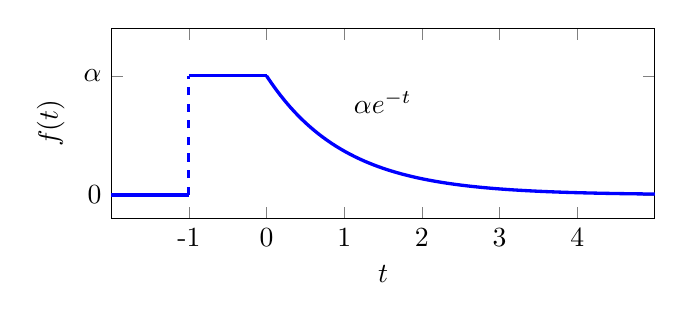
\begin{tikzpicture}
\begin{axis}[xmin= -2, xmax=5, ymin=-0.1, ymax=0.7, xlabel=$t$,
ylabel=$f_{\rt}(t)$,height=4cm,
width=0.7\textwidth,
xticklabels={-1,0,...,4}, xtick={-1,0,1,...,4},
yticklabels={0,$\alpha$}, ytick={0,0.5}]
%\addplot+[ycomb, blue, very thick, samples=2] coordinates {(0,1)(1,1)};
\addplot[blue, very thick, samples=2] coordinates {(-2,0)(-1,0)};
\addplot[blue, very thick, samples=2] coordinates {(-1,0.5)(0,0.5)};
%\addplot[dashed,blue, very thick, samples=2] coordinates {(0,0)(0,0.5)};
\addplot[dashed, blue, very thick, samples=2] coordinates {(-1,0)(-1,0.5)};
\addplot[blue, very thick, domain=0:6, samples=101] {0.5*exp(-x)};
\node at (axis cs:1,0.3) [anchor=south west] {$\alpha e^{-t}$};
%\addplot[dashed,blue, very thick, samples=2] coordinates {(0,0)(0,0.5)};
\end{axis}
\end{tikzpicture} 
\end{center}
\end{figure}\\
models the time at which there is a leak in a nuclear power plant. The pdf is constant during the time the station is built (between -1 and 0) and exponential with parameter 1 afterwards (from 0 to $+\infty$). 
\begin{enumerate}
\item Compute the value of the constant $\alpha$. 
\blue{
\begin{itemize}
    \item for this PDF to make sense it must be the case that $\int_{-1}^{0}\alpha dt+\int_{0}^{\infty}\alpha e^{-t} dt=1$ 
    \item we can see that $\int_{-1}^{0}\alpha dt+\int_{0}^{\infty}\alpha e^{-t} dt=\alpha|_{-1}^{0}-\alpha e^{-t}|_{0}^{\infty}=2\alpha$
    \item thus it must be the case that $2\alpha=1$ meanign that $\alpha=\frac{1}{2}$
\end{itemize}}
\item Compute the cdf of $\rt$ and plot it.
\blue{
\begin{itemize}
    \item the cdf is $F_\Tilde{T}(t)=P(\Tilde{t}\leq t)$
    \item if $t\leq -1$ $F_\Tilde{T}(t)=0$
    \item if $t\leq 0 and t\geq -1$ we know $F_\Tilde{T}(t)=\int_{-1}^{t}\frac{1}{2}du=\frac{1}{2}u|_{-1}^{t}=\frac{1+t}{2}$
    \item if $t \geq 0$ it must be the case that$F_\Tilde{T}(t)=\int_{-1}^{t}\frac{1}{2}du+\int_{0}^{\infty}\frac{1}{2}e^{-u}du=\frac{1}{2}|_{-1}^{0}+\frac{-1}{2}e^{-u}|_{0}^{t}=\frac{1}{2}-\frac{1}{2}e^{-u}|_{0}^{t}\\=1-\frac{1}{2}e^{-t}$
    \item so finally we see that $f_{\Tilde{t}}(t) = 
\left\{
    \begin{array}{lr}
        0, & \text{if } t \leq -1\\
        \frac{1+t}{2}, & \text{if } t\leq 0 \text{ and } t\geq -1\\
        1-\frac{1}{2}e^{-t}&  \text{ if } t\geq 0
        
    \end{array}$
    
    \includegraphics[width=15cm]{homework 3/question 2.png}
\end{itemize}
}

\item Compute the pdf of $\rt$ conditioned on $\rt <0$.
\blue{
\begin{itemize}
    \item first let us solve for the new cdf. 
    \item so we know we are looking for the likclyhood that $\Tilde{t}>y$ given t is less than 0 this can be expressed as $P(\Tilde{t}<y|\Tilde{y}<0)=\frac{P(\Tilde{t}<y \cap \Tilde{t}<0)}{P(\Tilde{t}<0)}=\frac{1-P(\Tilde{t}>y \cap \Tilde{t}<0)}{P(\Tilde{t}<0)}$ \item this can be expressed in terms of the cdf we already know as 
    $\frac{1-P(\Tilde{t}>y \cap \Tilde{t}<0)}{P(\Tilde{t}<0)}=\frac{1-(F_{\Tilde{t}}(0)-F_{\Tilde{t}}(y))}{F_{\Tilde{t}}(0)}=\frac{1-\frac{1}{2}+\frac{1+y}{2}}{\frac{1}{2}}=\frac{\frac{1}{2}+\frac{1+y}{2}}{\frac{1}{2}}=1+\frac{2(1+y)}{2}=2+y$ 
    \item we can call this new cdf $G_{\Tilde{t}}(y) = 
\left\{
    \begin{array}{lr}
        2+y, & \text{if } y\leq 0 \text{ and } y\geq -1\\
        0&  \text{otherwise }
    \end{array}$
    \item then we know that the pdf we are looking for is the darivative of this cdf so we can see that $g_{\Tilde{t}}(y)=\frac{dG_{\Tilde{t}(y)}}{dy}=\left\{
    \begin{array}{lr}
        1, & \text{if } y\leq 0 \text{ and } y\geq -1\\
        0&  \text{otherwise }
    \end{array}$
    \item then we can check that this is sensible as $\int_{\mathbb{R}}g{\Tilde{t}}(y)dy=\int_{-\infty}^{-1}0dy+\int_{-1}^{0}1dy+\int_{0}^{\infty}0dy=1$
    
\end{itemize}

}
\end{enumerate}
\newpage
\item (Measurements)  
You have access to the readings of a device that indicates whether a radioactive particle has decayed. However you do not get a continuous reading, you get a reading every second. 
\begin{enumerate}
\item A reasonable model for the time the particle takes to decay is that it is a random variable with pdf
\begin{align}
f_{\rnd{t}}(t) := \begin{cases}
$\lambda \exp(- \lambda t), \qquad \text{if $t\geq 0$},\\
0$ \qquad \text{otherwise},
\end{cases}
\end{align}
where $\lambda$ is a fixed constant. Taking into account that the measurement device rounds up the time and outputs an integer number of seconds (if the time is $0.1$ it outputs 1, if it is 13.4 it outputs 14), compute the pmf of the reading from the device. What kind of random variable is this? 
\blue{
\begin{itemize}
    \item let int(a) be the function that rounds the real numebr a up to the nearest integer
    \item we can see that $P(\Tilde{t}=x)=\int_{int(x-1)}^{int(x)}\lambda e^{-\lambda t}dt=-e^{-\lambda t}|_{int(x-1)}^{int(x)}\\=e^{-\lambda(int(x-1))}-e^{-\lambda(int(x))}$
    if $t\geq 0$ and 0 elsewhere
    \item this is gemoetric distrobutin 
    \item F_{\rnd{t}}(t) := \begin{cases}
$(1-e^{-\lambda})e^{-\lambda(t-1)}, \qquad \text{if $t\geq 0$},\\
0$ \qquad \text{otherwise},
\end{cases}
\end{itemize}
}
\item What is the pdf of the error between your reading and the true time of decay?
\blue{
\begin{itemize}
\item we must first deffine a few things.
\item \Tilde{R} be the random varible represneting the possible outcomes for the actual time decay 
\item let \Tilde{t} be the random varible represening our measurment 
\item let \Tilde{e}=\Tilde{t}-\Tilde{r} be the random varible represting the error
\item we can see that the cdf of the error is 
\item $F_\Tilde{e}(t)=P(\Tilde{e}\leq e)=P(\Tilde{t}-\Tilde{r}\leq e)$ we know that r can take on values between 1 and infinty units of time. so we can express this using a union of sets $P(\Tilde{t}-\Tilde{r}\leq e)=P(U_{r=1}^{\infty}\{\r-r\leq \Tilde{t}\leq r\})$ so we are looking at the the union of the liclyhood that t is in many disjoint intervals 
\item so we can express this as a sum of proabilit.es
\item that is $P(U_{r=1}^{\infty}\{r-e\leq \Tilde{t}\leq r\})=\sum_{r=1}^{\infty}P(r-e\leq \Tilde{t}\leq r)=\sum_{r=1}^{\infty}\int_{t-e}^tf\Tilde{t}(t)dt=\sum_{r=1}^{\infty}\int_{t-e}^t(1-e^{-\lambda})e^{-\lambda(t-1)}dt=\sum_{r=1}^{\infty}(e^-\lambda r)(e^{\lambda x}-1)=\frac{e^{\lambda y}-1}{e^{\lambda}-1}$
\item so finalyl we see that our Cdf is $F\Tilde{e}=\frac{e^{\lambda y}-1}{e^{\lambda}-1}$ if t is betwene 0 and 1 and 0 elsewhere 
\item so taking the davivative of the cdf we can see that the pdf is $f_t(t)=\frac{\lambda e^{\lambda t}}{e^{\lambda}-1 }$ if t is between 0 and 1 and 0 elsewhere 
\end{itemize}
}
\end{enumerate}
\newpage
\item (Applying the cdf) The array in \texttt{samples.npy} contains $n := 1,000$ i.i.d. samples from a certain distribution. 
\begin{enumerate}
\item Compute the empirical cdf of the data $F_X$ and plot it.
\blue{
\begin{itemize}
    \item \includegraphics[width=15cm]{homework 3/empircal question 3.png}
\end{itemize}
}

\item If you apply the empirical cdf to each data point $x_i$ , $1\leq i \leq n$, to obtain a new data point $y_i := F_X(x_i)$, what are the new data equal to? Does your answer depend on the distribution of the data?
\blue{
\begin{itemize}
    \item by theorem 3.23 we know that $y_i$ will be uniformly distributed regardless of the distribution of the data.
\end{itemize}


}
\end{enumerate}
\end{enumerate}
\end{document}
